\ps{I'm thinking an intro to globular clusters, then to modelling GCs with discussion of binaries,
	then to observations of binaries in GC}

\section{Globular Clusters}

Globular clusters (GCs) are dense, spheroidal collection of stars bound by their own self-gravity.
GCs are found in most galaxies and in the Milky Way are located both in the halo and the disk. GCs
typically represent some of the oldest stellar populations in the universe and are usually in excess
of 10 billion years old.

Mention mass segregation

\subsection{Binaries in Globular Clusters}

Mention why we expect binaries in GCs to be different from field binaries. (cite a field binary and GC binary paper here)

Some dynamical effects of binaries, mention that we're focusing on hard binaries that we can treat
as point masses, not so much the long-period binaries that provide significant energy through
hardening during interactions.

Check some of those "Binary Burning" papers.

\subsection{Observations of Binary Stars in Globular Clusters}

\paragraph{}
In general, there are three methods typically used to detect binaries within globular clusters:
high-precision photometry observations of main-sequence stars, radial velocity searches and
time-series photometry.

\paragraph{}
High-precision photometry can be used to detect binaries along the main sequence which have a
significant difference in the mass of their components ( typically these systems have a mass ratio,
$q$, larger than $0.5$). These systems will appear to be raised above the main-sequence when plotted
on a colour-magnitude diagram as their colour will match that of a typical main-sequence star
however their luminosity will be the sum of both components. Figure
\ref{fig:1/main_sequence_binaries} shows the main-sequence of the cluster NGC 2298, the binary stars
in this cluster are visible above the main-sequence according to their mass ratio.
\citet{Milone2012} performed high-precision photometry on several globular clusters using the Hubble
Space Telescope's (HST) Advanced Camera for Surveys and was able to place strong constraints on the
binary fraction for binaries with a mass ratio above $q=0.5$. This method allows for large studies
of binary populations in GCs without the need for dedicated observations but suffers from an
inherent bias towards systems with high mass ratios. Systems with mass ratios below $q=0.5$ are
typically too close to the regular main-sequence to confidently classify as binaries (see Figure
\ref{fig:1/main_sequence_binaries}). This means that studies which employ this method must assume an
underlying mass-ratio distribution if they wish to place any limits on the overall binary fraction
of a cluster.

\ps{Put fig 1 from milone2012 here}

\begin{figure}
	\centering
	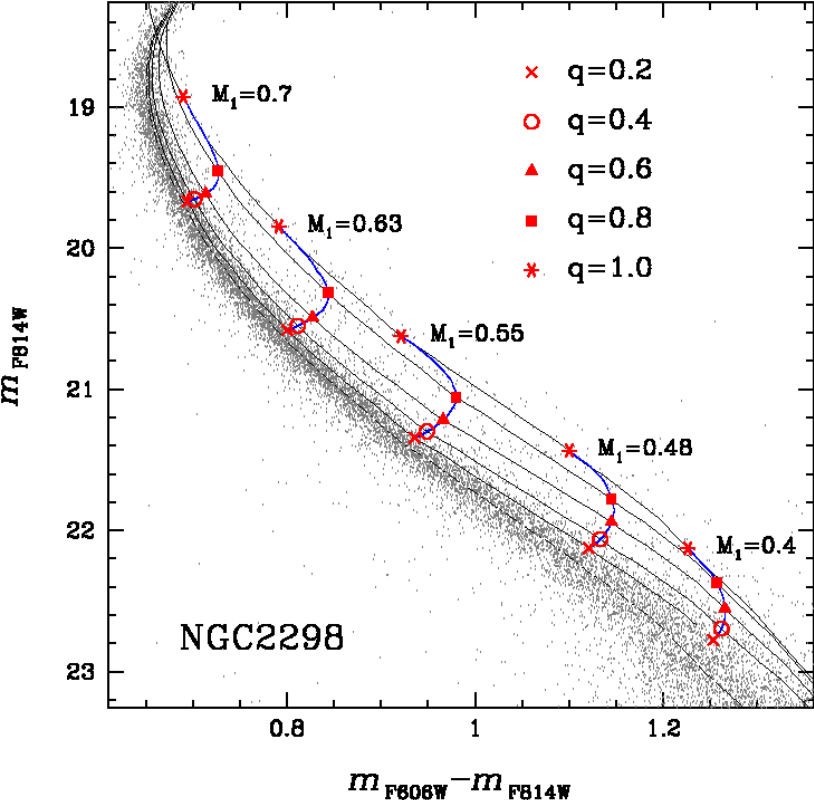
\includegraphics[width=0.8\textwidth]{"./figures/main_sequence_binaries.pdf"}
	\label{fig:1/main_sequence_binaries}
	\caption{Reproduced from Figure 1 of \citet{Milone2012}. Binaries are observed as being above the
		main-sequence of the cluster. Higher mass ratios are further above the main-sequence
		and smaller mass ratios are indistinguishable from the main-sequence.}
\end{figure}


Radical Velocity Searches \citet{Giesers2019}. Large-scale campaigns to measure the radial
velocities for many stars in a cluster over several epochs are another method which can be used to
detect binaries in GCs. Systems which are found to have periodically varying radial velocities can
typically be confidently classified as binary systems. \citet{Giesers2019} used the MUSE integral
field spectrograph installed at the European Southern Observatory's Very Large Telescope to observe
several GCs and reported the results for NGC 3201. Integral field spectrographs provide spatially
resolved spectra for the entire field of view of the detector which enables far more time-efficient
surveys than previous methods. Because this methods measure radial velocities and periods, it can be
used to constrain most of a binary system's orbital parameters allowing us to verify our assumptions
\ps{does it validate them? some binaries with periods up to 1000 days there?} about the period
distributions of binaries in globular clusters. \ps{grab a figure from the MUSE paper with period
distribution?}



\section{Modelling Globular Clusters}

\paragraph{}
When modelling globular clusters, there are generally two approaches you can take. The first is to
model the entire evolutionary history of the cluster from initial conditions to the present. The
most commonly employed versions of these "evolutionary models" are direct N-body integration (see
for example \citet{Baumgardt2017a}) which directly calculate the gravitational interactions between
each object in the cluster and Monte-Carlo models (see \citet{Rodriguez2021} or \cite{Hypki2013})
which approximate the gravitational interactions between object according to the method of
\citet{Henon1971}. While these models provide insight into the dynamical history of the cluster,
they are very computationally expensive with even the fastest models taking on the order of a day
to model a realistic globular cluster \citep{Rodriguez2021}.

The second approach is to model just the present-day conditions of the cluster.

DF models (LIMEPY \citet{Gieles2015})

